\documentclass{beamer}

% Theme and style
\usetheme{Madrid}
\usecolortheme{seahorse}
\setbeamertemplate{navigation symbols}{}
\setbeamertemplate{footline}[frame number]

% Packages
\usepackage{listings}
\usepackage{tikz} 
\usetikzlibrary{positioning}
\usepackage{graphicx}
\usepackage{hyperref}
\usepackage{amsmath}
\usepackage{caption}

% Listings setup for C code
\lstset{
  language=C,
  basicstyle=\ttfamily\footnotesize,
  keywordstyle=\color{blue},
  commentstyle=\color{gray},
  stringstyle=\color{red},
  showstringspaces=false,
  breaklines=true,
  frame=single,
  numbers=left,
  numberstyle=\tiny\color{gray}
}

% Title Info
\title[ESP ChatBot]{\textbf{ESP ChatBot: Offline-First Voice Interface on ESP32}}
\subtitle{Wake Word Detection, Audio Capture, and MQTT/HTTP Streaming}
\author{Abdul Baseer}
\institute{AI | Embedded AI | ESP32 Developer}
\date{\today}

% Document
\begin{document}

% Title Slide
\begin{frame}
  \titlepage
\end{frame}

% Outline
\begin{frame}{Agenda}
  \tableofcontents
\end{frame}

% Section 1
\section{Introduction}
\begin{frame}{What is ESP ChatBot?}
  \begin{itemize}
    \item Lightweight, offline-first voice interface framework
    \item Runs on ESP32-S3 with ESP-IDF v5.x
    \item Built on Espressif’s ESP-SR v2.0.5
    \item Detects custom wake word ``\textbf{hijason}''
    \item Captures audio from I2S microphone
    \item Publishes PCM audio via MQTT or HTTP
  \end{itemize}
\end{frame}
 
 
\section{Architecture}
\begin{frame}[fragile]{System Architecture} 
  \begin{columns} 
    \column{0.5\textwidth}
    \begin{itemize}
      \item Wake Word Detection: WakeNet9
      \item Audio Capture: I2S, 16kHz, PCM16
      \item Networking: MQTT / HTTP
      \item Modular components:
        \begin{itemize}
          \item \texttt{custom\_audio}
          \item \texttt{custom\_network}
          \item \texttt{custom\_system}
        \end{itemize}
    \end{itemize}

    \column{0.5\textwidth} 
    \centering % ✅ safe inside columns
    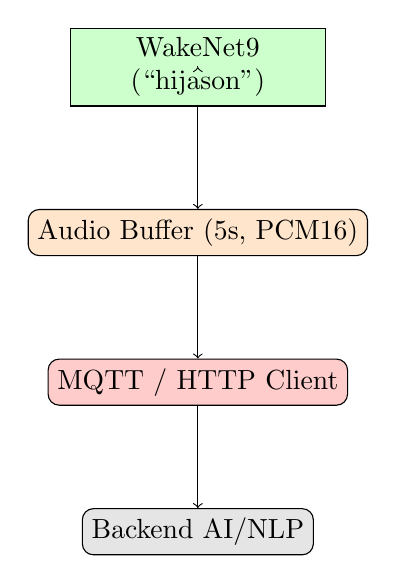
\begin{tikzpicture}[node distance=1.3cm, auto]
      \node[draw, rounded corners, fill=blue!20] (mic) {I2S Microphone};
     \node[draw, fill=green!20, text width=3cm, align=center] (wakenet) {WakeNet9 \\ (``hijason'')};
      \node[draw, rounded corners, below=of wakenet, fill=orange!20] (buffer) {Audio Buffer (5s, PCM16)};
      \node[draw, rounded corners, below=of buffer, fill=red!20] (net) {MQTT / HTTP Client};
      \node[draw, rounded corners, below=of net, fill=gray!20] (server) {Backend AI/NLP};

      \draw[->] (mic) -- (wakenet);
      \draw[->] (wakenet) -- (buffer);
      \draw[->] (buffer) -- (net);
      \draw[->] (net) -- (server);
    \end{tikzpicture}
  \end{columns} 
\end{frame}


% Section 3
\section{Wake Word Detection}
\begin{frame}[fragile]{Wake Word Detection}
  \begin{itemize}
    \item Model: WakeNet9
    \item Custom keyword: \textbf{``hijason''}
    \item Model stored as binary array in flash (\texttt{hijason.h})
  \end{itemize}

  \vspace{5mm}
  \textbf{Integration Example:}
  \begin{lstlisting}
// Reference to WakeNet9 model
const esp_wn_iface_t *wn_iface = &ESP_WN9_MODEL;
model_iface_data_t *wn_model = (model_iface_data_t *)&hijason;

// Start Wake Word Detection
wn_iface->create(wn_model);
wn_iface->detect(wn_model, audio_buffer);
  \end{lstlisting}
\end{frame}

% Section 4
\section{Audio Pipeline}
\begin{frame}{Audio Pipeline}
  \begin{itemize}
    \item Captures 5 seconds of audio after wake word detection
    \item Mono, 16-bit, 16kHz sampling
    \item Stored in ring buffer
    \item Processed asynchronously via FreeRTOS tasks
  \end{itemize}
  
  \vspace{5mm}
  \textbf{Pipeline Flow:}
  \begin{center}
  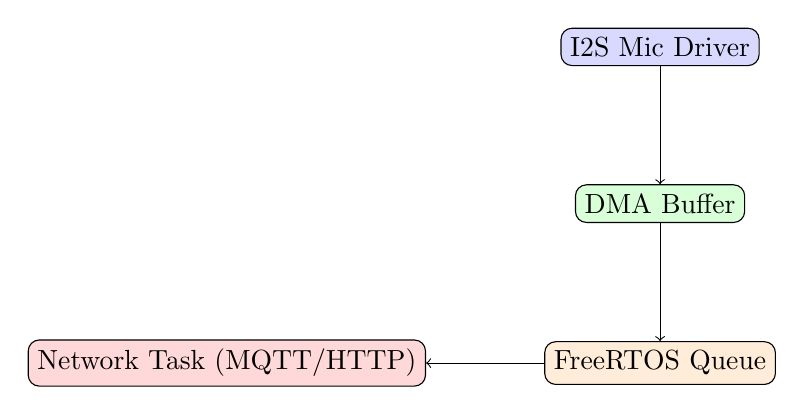
\begin{tikzpicture}[node distance=1.5cm, auto]
    \node[draw, fill=blue!15, rounded corners] (mic) {I2S Mic Driver};
    \node[draw, fill=green!15, below=of mic, rounded corners] (dma) {DMA Buffer};
    \node[draw, fill=orange!15, below=of dma, rounded corners] (queue) {FreeRTOS Queue};
    \node[draw, fill=red!15, left=of queue, rounded corners] (net) {Network Task (MQTT/HTTP)};
    
    \draw[->] (mic) -- (dma);
    \draw[->] (dma) -- (queue);
    \draw[->] (queue) -- (net);
  \end{tikzpicture}
  \end{center}
\end{frame}

% Section 5
\section{Networking}
\begin{frame}[fragile]{Networking}
  \begin{itemize}
    \item Sends audio buffer to backend server
    \item Protocols: MQTT or HTTP
  \end{itemize}

  \vspace{5mm}
  \textbf{MQTT Example:}
  \begin{lstlisting}
// Publish PCM audio
esp_mqtt_client_publish(client,
    "esp/audio/hijason",
    (const char *)pcm_buffer,
    buffer_size, 0, 0);
  \end{lstlisting}

  \textbf{HTTP Example:}
  \begin{lstlisting}
POST /api/audio HTTP/1.1
Content-Type: audio/raw
Body: [binary PCM16LE data]
  \end{lstlisting}
\end{frame}

% Section 6
\section{Performance and Security}
\begin{frame}{Performance \& Security}
  \begin{block}{Performance}
    \begin{itemize}
      \item WakeNet9 on ESP32-S3:
      \item $\sim$28\% average CPU load
      \item $\sim$39\% peak CPU usage
      \item Optimized FreeRTOS task priorities
    \end{itemize}
  \end{block}
  \begin{block}{Security}
    \begin{itemize}
      \item MQTT not encrypted by default
      \item Recommend TLS + authentication
      \item Always validate audio buffer bounds
    \end{itemize}
  \end{block}
\end{frame}

% Section 7
\section{Future Enhancements}
\begin{frame}{Future Enhancements}
  \begin{itemize}
    \item On-device Multinet for offline command recognition
    \item Lightweight TensorFlow Lite STT pipeline
    \item TTS playback (voice responses)
    \item Power management: light sleep between detections
  \end{itemize}
\end{frame}

% Section 8
\section{Conclusion}
\begin{frame}{Conclusion}
  \begin{itemize}
    \item ESP ChatBot enables low-power, offline-first voice interfaces
    \item WakeNet9 + ESP32-S3 = reliable wake word detection
    \item Modular design for easy integration with AI backends
    \item Flexible networking via MQTT and HTTP
  \end{itemize}

  \vspace{5mm}
  \centering
  \textbf{Questions?}
\end{frame}

\end{document}
